\documentclass[pdftex,12pt,xcolor=svgnames]{beamer}

\mode<presentation>
{
  \usetheme{boxes}
  \usecolortheme[named=MidnightBlue]{structure}
  %\setbeamercolor{normal text}{bg=NavajoWhite!20}
  \usefonttheme{serif}
  \setbeamertemplate{navigation symbols}{}
  % Show frame number and author name in footline
  \setbeamertemplate{footline}[frame number]
  \addtobeamertemplate{footline}{\quad\textcolor{gray}{James Robert Lloyd}}{}
  % Set frame titles in small capitals
  \setbeamerfont{frametitle}{shape=\scshape,family=\rmfamily}
  \setbeamercolor{frametitle}{bg=gray!60!white,fg=black}
  % Alerted text: blue (uncomment second line if theme sets alerted text to bold)
  \setbeamercolor{alerted text}{fg=blue}
  %\setbeamerfont*{alerted text}{}
  \setbeamertemplate{bibliography item}[text] %{\hbox{\donotcoloroutermaths$\blacktriangleright$}}
  \setbeamertemplate{bibliography entry title}{}
  \setbeamertemplate{bibliography entry author}{}
  \setbeamertemplate{bibliography entry note}{}
  \setbeamertemplate{bibliography entry location}{}

}
\usepackage[english]{babel}
\usepackage[latin1]{inputenc}
\usepackage{times}
\usepackage[T1]{fontenc}
\usepackage{hyperref}
\usepackage{multimedia}
\usepackage{eepic}
\usepackage{graphicx}
%\usepackage[nohug]{latexinclude/diagrams}
\usepackage{tikz}
\usetikzlibrary{calc}

%% \newcommand{\footlineextra}[1]{
%%     \begin{tikzpicture}[remember picture,overlay]
%%         \node[yshift=1.5ex,anchor=south east] at (current page.south east)
%% {#1};
%%     \end{tikzpicture}
%% }

\newcommand{\footlineextra}[1]{
    \begin{tikzpicture}[remember picture,overlay]
        \node[xshift=-5ex,yshift=-0.5ex,anchor=south east] at (current page.south east)
             {\mbox{\tiny \textcolor{MidnightBlue}{#1}}};
    \end{tikzpicture}
}

\def\sectionframe#1{
  {
    \setbeamertemplate{footline}{\empty}
    \begin{frame}{}
      \begin{center}
        \huge\sc #1
      \end{center}
    \end{frame}
  }
}


\usepackage{etex}

\usepackage{tabularx}
\usepackage{include/picins}
\usepackage{include/preamble}
\usepackage{setspace}
\usepackage{xcolor}
\usepackage{tikz}

\usetikzlibrary{shapes.geometric,arrows,chains,matrix,positioning,scopes,calc,shapes.arrows}

%%%%%%%%%%%%%%%%%%%%%%%%%%%%%%%%%%%%%%%%%%%
%
% Some look and feel definitions
%
%%%%%%%%%%%%%%%%%%%%%%%%%%%%%%%%%%%%%%%%%%%

\setlength{\columnsep}{0.03\textwidth}
\setlength{\columnseprule}{0.0018\textwidth}
\setlength{\parindent}{0.0cm}
  
\tikzstyle{mybox} = [draw=white, rectangle]
\tikzset{hide on/.code={\only<#1>{\color{white}}}}

\definecolor{camlightblue}{rgb}{0.601 , 0.8, 1}
\definecolor{camdarkblue}{rgb}{0, 0.203, 0.402}
\definecolor{camred}{rgb}{1, 0.203, 0}
\definecolor{camyellow}{rgb}{1, 0.8, 0}
\definecolor{lightblue}{rgb}{0, 0, 0.80}
\definecolor{white}{rgb}{1, 1, 1}
\definecolor{whiteblue}{rgb}{0.80, 0.80, 1}

\newcolumntype{x}[1]{>{\centering\arraybackslash\hspace{0pt}}m{#1}}
\newcommand{\tabbox}[1]{#1}

\hypersetup{colorlinks=true,citecolor=blue}

%%%%%%%%%%%%%%%%%%%%%%%%%%%%%%%%%%%%%%%%%%%
%
% The talk
%
%%%%%%%%%%%%%%%%%%%%%%%%%%%%%%%%%%%%%%%%%%%

\title{Automatic Construction and Natural-Language Description of Nonparametric Regression Models}

\author{
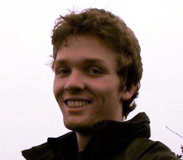
\includegraphics[height=0.16\textwidth]{figures/JamesLloyd4}
\qquad
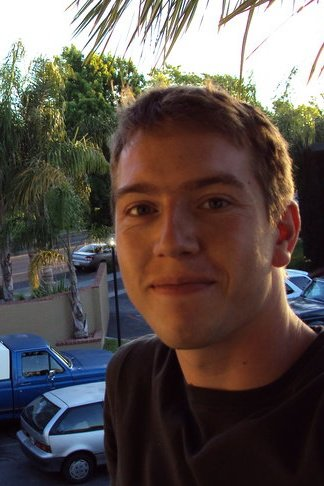
\includegraphics[height=0.16\textwidth, trim=20mm 25mm 0mm 25mm, clip]{figures/david2}
\qquad
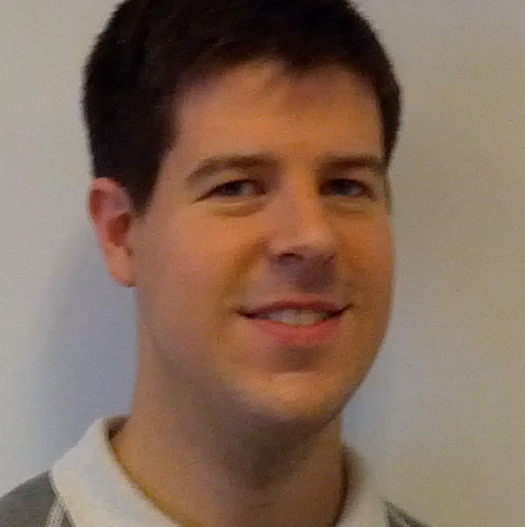
\includegraphics[height=0.16\textwidth]{figures/roger-photo}
\\
James Robert Lloyd\textsuperscript{1}, David Duvenaud\textsuperscript{1}, Roger Grosse\textsuperscript{2},\\
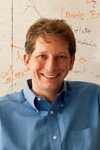
\includegraphics[height=0.16\textwidth, trim=0mm 7mm 0mm 0mm, clip]{figures/josh2}
\qquad
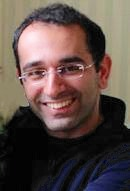
\includegraphics[height=0.16\textwidth]{figures/zg2}\\
Joshua Tenenbaum\textsuperscript{2}, Zoubin Ghahramani\textsuperscript{1}
}

\institute{
1: Department of Engineering, University of Cambridge, UK\\2: Massachusetts Institute of Technology, USA
}

\begin{document}

\frame[plain] {
\titlepage
}

\begin{frame}{A system for automatic data analysis}
    % Define block styles
  \tikzstyle{block} = [rectangle, draw, fill=blue!20, 
                       text width=4.4em, text centered, rounded corners, minimum height=3em]
  \tikzstyle{line} = [draw, -latex']
  \tikzstyle{cloud} = [draw, ellipse,fill=red!20,minimum height=2em]
    
  \begin{tikzpicture}[node distance = 2.3cm]
    \footnotesize
    % Place nodes
    \node [cloud] (data) {Data};
    \node [block, right of=data] (search) {Search};
    \node [cloud, above of=search] (language) {Language of models};
    \node [block, below of=search] (eval) {Evaluation};
    \node [cloud, right of=search] (model) {Model};
    \node [block, right of=model] (pred) {Prediction};
    \node [block, above of=pred] (trans) {Description};
    \node [block, below of=pred] (checking) {Checking};
    \node [cloud, right of=pred] (report) {Report};
    % Draw edges
    \path [line] (data) -- (search);
    \path [line] (language) -- (search);
    \path [line] (search) -- (model);
    \path [line] (search) -- (model);
    \path [line] (model.north east) -- (trans.south west);
    \path [line] (model.east) -- (pred.west);
    \path [line] (model.south east) -- (checking.north west);
    \path [line] (trans.south east) -- (report.north west);
    \path [line] (pred.east) -- (report.west);
    \path [line] (checking.north east) -- (report.south west);
    \draw[->,] (search.south east) .. controls (3.45,-1.15) .. (eval.north east);
    \draw[->,] (eval.north west) .. controls (1.15,-1.15) .. (search.south west);
  \end{tikzpicture}
\end{frame}

\begin{frame}{An entirely automatic analysis}
  \begin{center}
    \begin{tikzpicture}
      \begin{scope}[yshift=0\textwidth]
        \node (raw_data) at (-0.25\textwidth, 0) {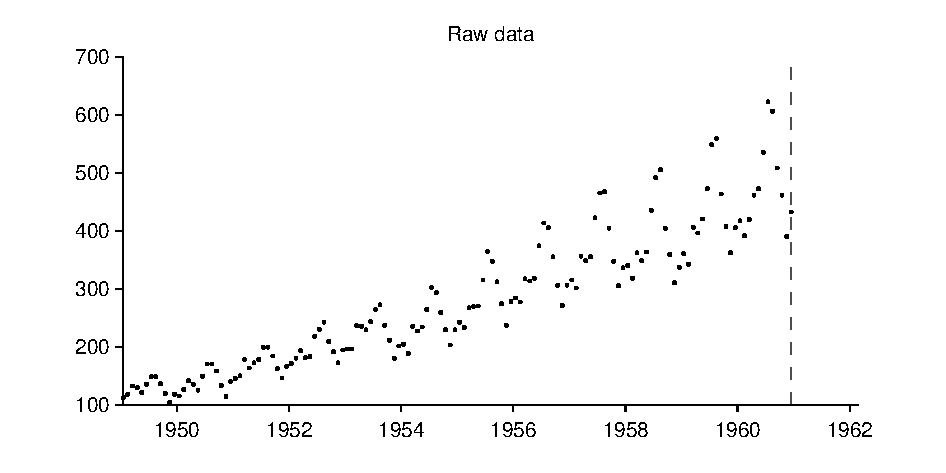
\includegraphics[width=0.45\textwidth]{figures/01-airline/01-airline_raw_data}};
        \node (posterior) at (+0.25\textwidth, 0)  {\includegraphics[width=0.45\textwidth]{figures/01-airline/01-airline_all}};
      \end{scope}
      \begin{scope}[yshift=-0.18\textwidth]
        \node (description) at (0, +0.03\textwidth) {\small Four additive components have been identified in the data};
        \node (component_1) at (-0.20\textwidth, -0.09\textwidth) 
              {\includegraphics[width=0.25\textwidth]{figures/01-airline/01-airline_1}};
        \node [text width=0.4\textwidth, align=center] (component_1_text) at (-0.20\textwidth, -0.193\textwidth) 
              {\scriptsize A linearly increasing function};
        \node (component_2) at (+0.20\textwidth, -0.09\textwidth) 
              {\includegraphics[width=0.25\textwidth]{figures/01-airline/01-airline_2}};
        \node [text width=0.4\textwidth, align=center] (component_2_text) at (+0.20\textwidth, -0.166\textwidth) 
              {\scriptsize An approximately periodic function};
        \node [text width=0.4\textwidth, align=center] (component_2_text) at (+0.20\textwidth, -0.193\textwidth) 
              {\scriptsize with a period of 1.0 years with};
        \node [text width=0.4\textwidth, align=center] (component_2_text) at (+0.20\textwidth, -0.220\textwidth) 
              {\scriptsize linearly increasing amplitude};
        \node (component_3) at (-0.20\textwidth, -0.3\textwidth) 
              {\includegraphics[width=0.25\textwidth]{figures/01-airline/01-airline_3}};
        \node [text width=0.4\textwidth, align=center] (component_3_text) at (-0.20\textwidth, -0.393\textwidth) 
              {\scriptsize A smooth function};
        \node (component_4) at (+0.20\textwidth, -0.3\textwidth) 
              {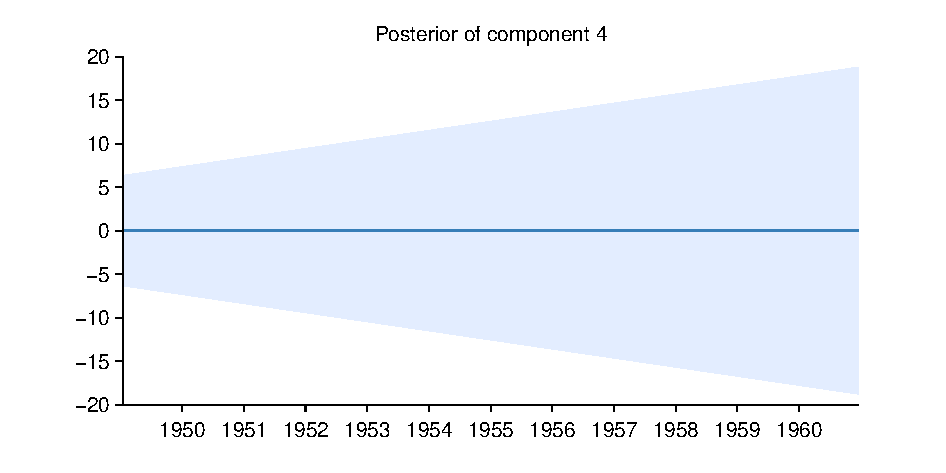
\includegraphics[width=0.25\textwidth]{figures/01-airline/01-airline_4}};
        \node [text width=0.4\textwidth, align=center] (component_4_text) at (+0.20\textwidth, -0.3795\textwidth) 
              {\scriptsize Uncorelated noise with linearly};
        \node [text width=0.4\textwidth, align=center] (component_4_text) at (+0.20\textwidth, -0.4065\textwidth) 
              {\scriptsize increasing standard deviation};
      \end{scope}
    \end{tikzpicture}
  \end{center}
\end{frame}

\begin{frame}{Natural language descriptions of models}
  \begin{center}
    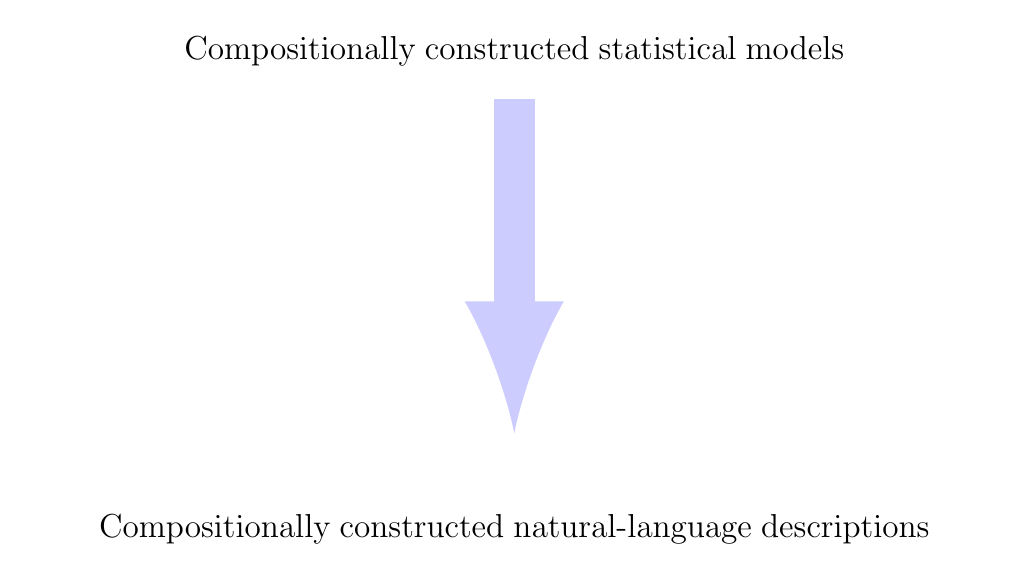
\begin{tikzpicture}
      \node (top_text) [text width=\textwidth, align=center] at (0, 0) {\large Compositionally constructed statistical models};
      \draw [->, >=latex, blue!20!white, line width=15pt] (0, -0.05\textwidth) to (0, -0.4\textwidth);
      \node (bottom_text) [text width=\textwidth, align=center] at (0, -0.5\textwidth) 
      {\large Compositionally constructed natural-language descriptions};
    \end{tikzpicture}
  \end{center}
\end{frame}

\begin{frame}{Defining a language of models}
    % Define block styles
  \tikzstyle{block} = [rectangle, draw, fill=blue!20, 
                       text width=4.4em, text centered, rounded corners, minimum height=3em]
  \tikzstyle{line} = [draw, -latex']
  \tikzstyle{cloud} = [draw, ellipse,fill=red!20,minimum height=2em]
  \tikzstyle{supercloud} = [draw, ellipse,fill=red!50,minimum height=2em,]
    
  \begin{tikzpicture}[node distance = 2.3cm]
    \footnotesize
    % Place nodes
    \node [cloud] (data) {Data};
    \node [block, right of=data] (search) {Search};
    \node [supercloud, above of=search] (language) {\bf Language of models};
    \node [block, below of=search] (eval) {Evaluation};
    \node [cloud, right of=search] (model) {Model};
    \node [block, right of=model] (pred) {Prediction};
    \node [block, above of=pred] (trans) {Description};
    \node [block, below of=pred] (checking) {Checking};
    \node [cloud, right of=pred] (report) {Report};
    % Draw edges
    \path [line] (data) -- (search);
    \path [line] (language) -- (search);
    \path [line] (search) -- (model);
    \path [line] (search) -- (model);
    \path [line] (model.north east) -- (trans.south west);
    \path [line] (model.east) -- (pred.west);
    \path [line] (model.south east) -- (checking.north west);
    \path [line] (trans.south east) -- (report.north west);
    \path [line] (pred.east) -- (report.west);
    \path [line] (checking.north east) -- (report.south west);
    \draw[->,] (search.south east) .. controls (3.45,-1.15) .. (eval.north east);
    \draw[->,] (eval.north west) .. controls (1.15,-1.15) .. (search.south west);
  \end{tikzpicture}
\end{frame}

\begin{frame}{A language of Gaussian processes}
  \begin{itemize}
    \item Define probability distributions on functions
    \item Used to perform Bayesian (nonlinear) regression
  \end{itemize}
  \vspace{\baselineskip}
  \begin{center}
    \includegraphics<1>[width=0.8\textwidth]{figures/lin_reg/sq_exp_prior}
    \includegraphics<2>[width=0.8\textwidth]{figures/quad/sq_exp_1}
    \includegraphics<3>[width=0.8\textwidth]{figures/quad/sq_exp_2}
    \includegraphics<4>[width=0.8\textwidth]{figures/quad/sq_exp_3}
    \includegraphics<5>[width=0.8\textwidth]{figures/quad/sq_exp_5}
    \includegraphics<6>[width=0.8\textwidth]{figures/quad/sq_exp_10}
    \includegraphics<7>[width=0.8\textwidth]{figures/quad/sq_exp_15}
  \end{center}
\end{frame}

\begin{frame}{The atoms of our language}  
  \newcommand{\fhbig}{1.0cm}
\newcommand{\fwbig}{1.2cm}
\newcommand{\kernpic}[1]{\includegraphics[height=\fhbig,width=\fwbig]{../figures/structure_examples/#1}}
\newcommand{\colsize}{1.7cm}
\newcommand{\sepsize}{0.0cm}

Five base kernels\dots

\vspace{\baselineskip}

\begin{tabularx}{\columnwidth}{x{\colsize}x{\colsize}x{\colsize}x{\colsize}x{\colsize}}
  \kernpic{se_kernel} & \kernpic{per_kernel} & \kernpic{lin_kernel} & \kernpic{c_kernel} & \kernpic{wn_kernel} \\
  {\footnotesize Squared \newline exp. (\kSE)} & {\footnotesize Periodic (\kPer)} & {\footnotesize Linear (\kLin)} & {\footnotesize Constant (\kC)} & {\footnotesize White \newline noise (\kWN)}
\end{tabularx}

\vspace{\baselineskip}

\dots encoding for the following types of functions

\vspace{\baselineskip}

\begin{tabularx}{\columnwidth}{x{\colsize}x{\colsize}x{\colsize}x{\colsize}x{\colsize}}
  \kernpic{se_kernel_draws} & \kernpic{per_kernel_draws_s2} & \kernpic{lin_kernel_draws} & \kernpic{c_kernel_draws} & \kernpic{wn_kernel_draws} \\
  {\footnotesize Smooth \newline functions} & {\footnotesize Periodic functions} & {\footnotesize Linear \newline functions} & {\footnotesize Constant \newline functions} & {\footnotesize Gaussian \newline noise} 
\end{tabularx}


\end{frame}

\begin{frame}{The composition rules of our language}
\begin{itemize} 
	\item Two main operations: addition, multiplication
\end{itemize}
\newcommand{\fhbig}{1.6cm}
\newcommand{\fwbig}{1.8cm}
\newcommand{\kernpic}[1]{\includegraphics[height=\fhbig,width=\fwbig]{figures/structure_examples/#1}}
\newcommand{\largeplus}{\tabbox{{\Large+}}}
\newcommand{\largeeq}{\tabbox{{\Large=}}}
\newcommand{\largetimes}{\tabbox{{\Large$\times$}}}
\begin{figure}[ht]
\centering
\renewcommand{\tabularxcolumn}[1]{>{\arraybackslash}m{#1}}
\begin{tabularx}{\columnwidth}{XXcXX}
  {\small $\kLin \times \kLin$} & \kernpic{lin_times_lin_draws} & \phantom{mm}
& {\small $\kSE \times \kPer$} & \kernpic{longse_times_per_draws_s1}
\\
   & {\small quadratic functions} & \phantom{mm}
&  & {\small locally \newline periodic}
\\ \\
%\midrule 
  {\small $\kLin + \kPer$} & \kernpic{lin_plus_per_draws} & \phantom{mm} 
& {\small $\kSE + \kPer$ } & \kernpic{se_plus_per_draws_s7}
\\
   & {\small periodic plus linear trend} & \phantom{mm}
&  & {\small periodic plus smooth trend}
\end{tabularx}
\end{figure}


\end{frame}

\begin{frame}{Automatic translation of models}
    % Define block styles
  \tikzstyle{block} = [rectangle, draw, fill=blue!20, 
                       text width=4.4em, text centered, rounded corners, minimum height=3em]
  \tikzstyle{superblock} = [rectangle, draw, fill=blue!50, 
                       text width=4.4em, text centered, rounded corners, minimum height=3em]
  \tikzstyle{line} = [draw, -latex']
  \tikzstyle{cloud} = [draw, ellipse,fill=red!20,minimum height=2em]
  \tikzstyle{supercloud} = [draw, ellipse,fill=red!50,minimum height=2em]
    
  \begin{tikzpicture}[node distance = 2.3cm]
    \footnotesize
    % Place nodes
    \node [cloud] (data) {Data};
    \node [block, right of=data] (search) {Search};
    \node [cloud, above of=search] (language) {Language of models};
    \node [block, below of=search] (eval) {Evaluation};
    \node [cloud, right of=search] (model) {Model};
    \node [block, right of=model] (pred) {Prediction};
    \node [superblock, above of=pred] (trans) {Translation};
    \node [block, below of=pred] (checking) {Checking};
    \node [cloud, right of=pred] (report) {Report};
    % Draw edges
    \path [line] (data) -- (search);
    \path [line] (language) -- (search);
    \path [line] (search) -- (model);
    \path [line] (search) -- (model);
    \path [line] (model.north east) -- (trans.south west);
    \path [line] (model.east) -- (pred.west);
    \path [line] (model.south east) -- (checking.north west);
    \path [line] (trans.south east) -- (report.north west);
    \path [line] (pred.east) -- (report.west);
    \path [line] (checking.north east) -- (report.south west);
    \draw[->,] (search.south east) .. controls (3.45,-1.15) .. (eval.north east);
    \draw[->,] (eval.north west) .. controls (1.15,-1.15) .. (search.south west);
  \end{tikzpicture}
\end{frame}

\begin{frame}{Sums of kernels are sums of functions}
  If ${\textcolor{red}{f_1} \,\sim\, \gp{}(0, \textcolor{red}{\kernel_1})}$ and independently ${\textcolor{blue}{f_2} \,\sim\, \gp{}(0, \textcolor{blue}{\kernel_2})}$ then
  \begin{align*}
  \textcolor{red}{f_1} + \textcolor{blue}{f_2} \,\sim\, \gp{}(0, \textcolor{red}{\kernel_1} + \textcolor{blue}{\kernel_2})
  \end{align*}
  
\eg

\vspace{\baselineskip}

\begin{tabular}{ccccccc}
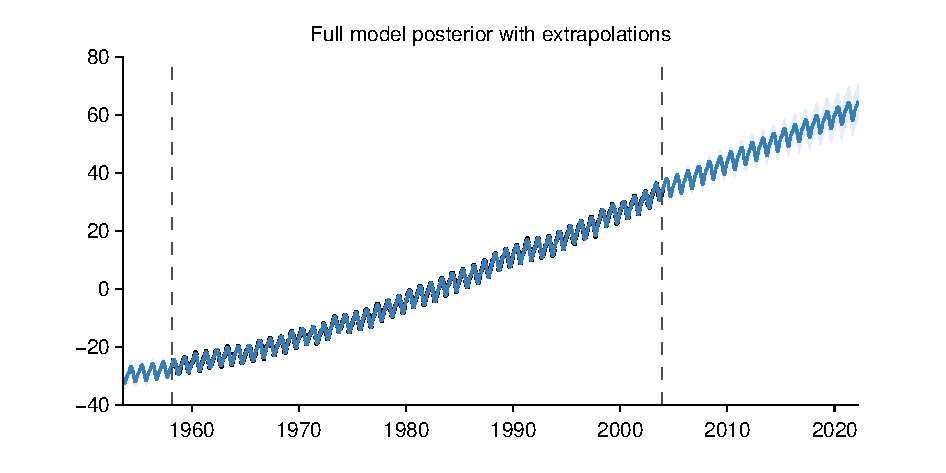
\includegraphics[trim=30 0 62 25, clip, width=0.15\textwidth]{figures/03-mauna2003_all} &
\raisebox{0.4cm}{$=$} &
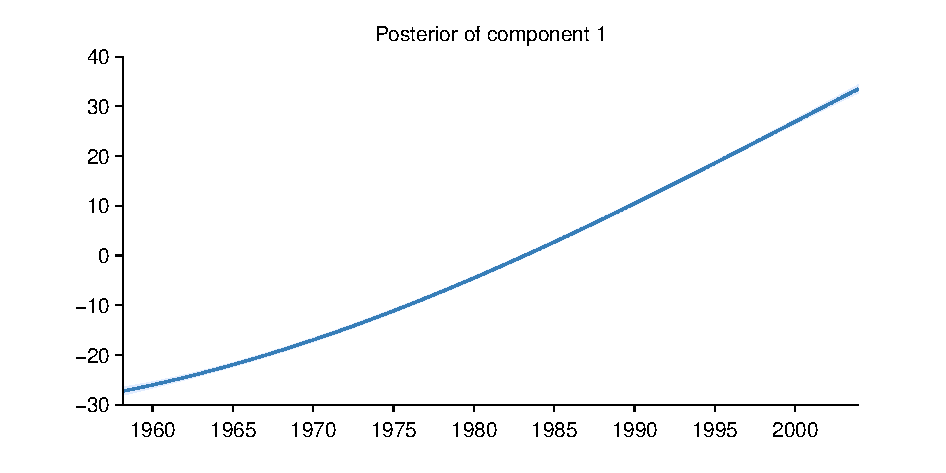
\includegraphics[trim=30 0 62 25, clip, width=0.15\textwidth]{figures/03-mauna2003_1} &
\raisebox{0.4cm}{$+$} &
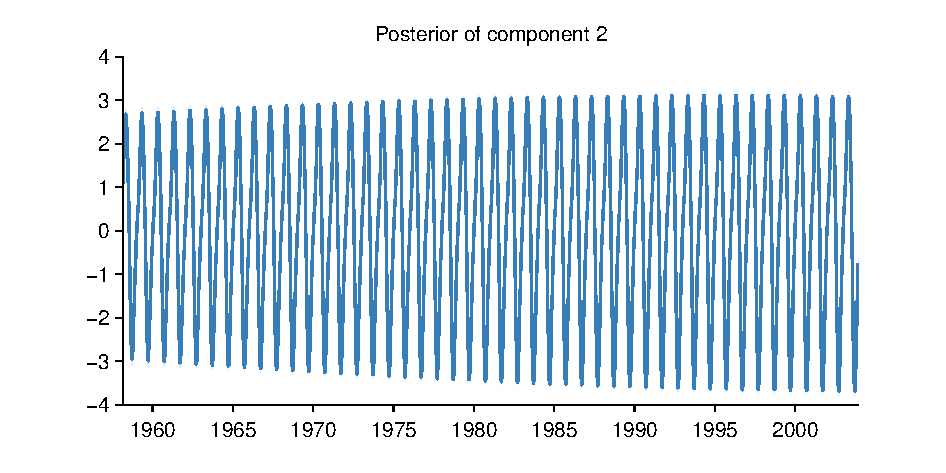
\includegraphics[trim=30 0 62 25, clip, width=0.15\textwidth]{figures/03-mauna2003_2} &
\raisebox{0.4cm}{$+$} &
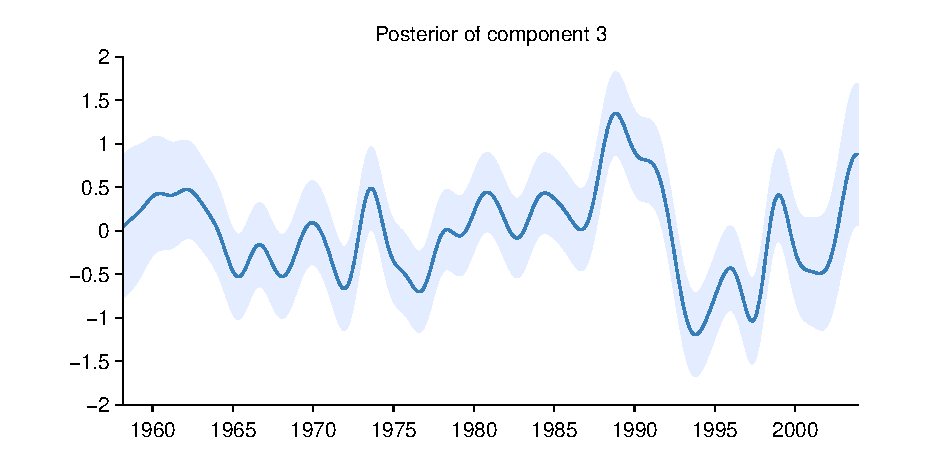
\includegraphics[trim=30 0 62 25, clip, width=0.15\textwidth]{figures/03-mauna2003_3}
\end{tabular}

\vspace{\baselineskip}

\begin{tabular}{ccccccc}
\includegraphics[trim=30 0 62 25, clip, width=0.15\textwidth]{figures/01-airline_all} &
\raisebox{0.4cm}{$=$} &
\includegraphics[trim=30 0 62 25, clip, width=0.15\textwidth]{figures/01-airline_1} &
\raisebox{0.4cm}{$+$} &
\includegraphics[trim=30 0 62 25, clip, width=0.15\textwidth]{figures/01-airline_2} &
\raisebox{0.4cm}{$+$} &
\includegraphics[trim=30 0 62 25, clip, width=0.15\textwidth]{figures/01-airline_3}
\end{tabular}

\vspace{\baselineskip}

We can therefore describe each component separately

\end{frame}

\begin{frame}{Products of kernels}
  \begin{align*}
    \phantom{\underbrace{\kSE}_{\textnormal{\scriptsize approximately}} \times }
    \underbrace{\kPer}_{\textnormal{\scriptsize periodic function}} \phantom{\times 
    \underbrace{\kLin}_{\textnormal{\scriptsize with linearly growing amplitude}} \times 
    \underbrace{\boldsymbol{\sigma}}_{\textnormal{\scriptsize until 1700}}}
  \end{align*}
  
  \vspace{\baselineskip}
  
  \begin{itemize}
  	\item Properties of individual kernels well understood
	\item Can be described with standard noun phrase
  \end{itemize}
  
  \vspace{\baselineskip}
  
  \begin{block}{}
    \begin{tabular}{cccc}
      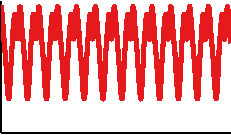
\includegraphics[width=0.2\textwidth]{figures/trans_samples/draw_11} &
      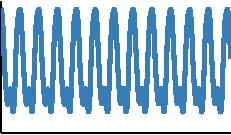
\includegraphics[width=0.2\textwidth]{figures/trans_samples/draw_12} &
      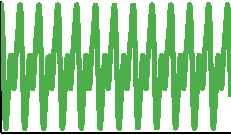
\includegraphics[width=0.2\textwidth]{figures/trans_samples/draw_13} &
      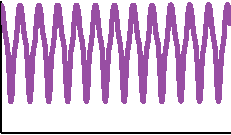
\includegraphics[width=0.2\textwidth]{figures/trans_samples/draw_14}
    \end{tabular}
  \end{block}
\end{frame}

\begin{frame}{Products of kernels}
  \begin{align*}
    \underbrace{\kSE}_{\textnormal{\scriptsize approximately}} \times
    \underbrace{\kPer}_{\textnormal{\scriptsize periodic function}} \phantom{\times 
    \underbrace{\kLin}_{\textnormal{\scriptsize with linearly growing amplitude}} \times 
    \underbrace{\boldsymbol{\sigma}}_{\textnormal{\scriptsize until 1700}}}
  \end{align*}
  
  \vspace{\baselineskip}
  
  \begin{itemize}
  	\item Multiplying by each kernel has a consistent effect
	\item Can be described with consistent adjectives / modifiers
  \end{itemize}
  
  \vspace{\baselineskip}
  
  \begin{block}{}
    \begin{tabular}{cccc}
      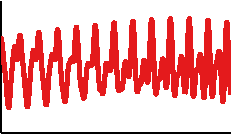
\includegraphics[width=0.2\textwidth]{figures/trans_samples/draw_21} &
      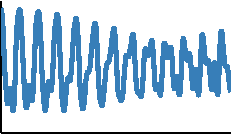
\includegraphics[width=0.2\textwidth]{figures/trans_samples/draw_22} &
      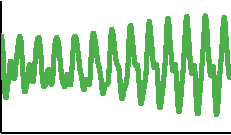
\includegraphics[width=0.2\textwidth]{figures/trans_samples/draw_23} &
      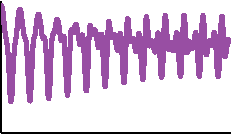
\includegraphics[width=0.2\textwidth]{figures/trans_samples/draw_24}
    \end{tabular}
  \end{block}
\end{frame}

\begin{frame}{Products of kernels}
  \begin{align*}
    \underbrace{\kSE}_{\textnormal{\scriptsize approximately}} \times
    \underbrace{\kPer}_{\textnormal{\scriptsize periodic function}} \times 
    \underbrace{\kLin}_{\textnormal{\scriptsize with linearly growing amplitude}} \phantom{\times 
    \underbrace{\boldsymbol{\sigma}}_{\textnormal{\scriptsize until 1700}}}
  \end{align*}
  
  \vspace{\baselineskip}
  
  \begin{itemize}
  	\item Multiplying by each kernel has a consistent effect
	\item Can be described with consistent adjectives / modifiers
  \end{itemize}
  
  \vspace{\baselineskip}
  
  \begin{block}{}
    \begin{tabular}{cccc}
      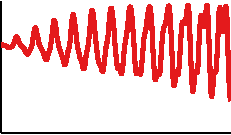
\includegraphics[width=0.2\textwidth]{figures/trans_samples/draw_31} &
      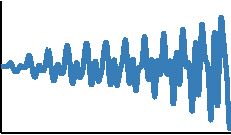
\includegraphics[width=0.2\textwidth]{figures/trans_samples/draw_32} &
      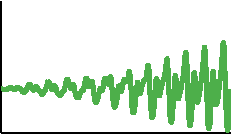
\includegraphics[width=0.2\textwidth]{figures/trans_samples/draw_33} &
      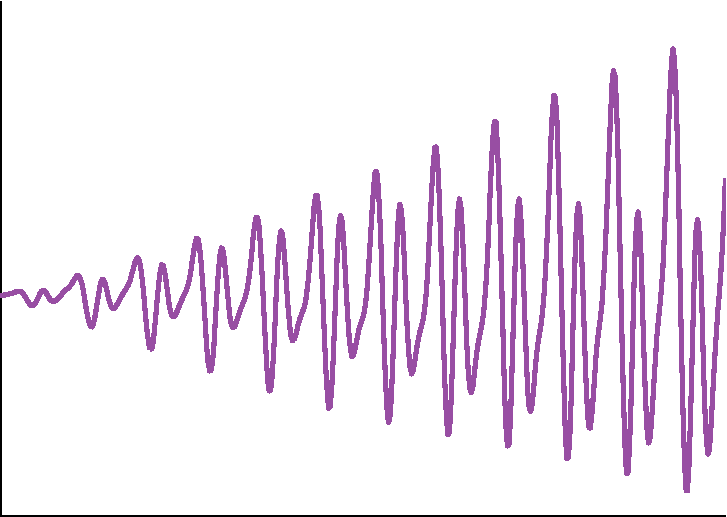
\includegraphics[width=0.2\textwidth]{figures/trans_samples/draw_34}
    \end{tabular}
  \end{block}
\end{frame}

\begin{frame}{Products of kernels}
  \begin{align*}
    \underbrace{\kSE}_{\textnormal{\scriptsize approximately}} \times
    \underbrace{\kPer}_{\textnormal{\scriptsize periodic function}} \times 
    \underbrace{\kLin}_{\textnormal{\scriptsize with linearly growing amplitude}} \times 
    \underbrace{\boldsymbol{\sigma}}_{\textnormal{\scriptsize until 1700}}
  \end{align*}
  
  \vspace{\baselineskip}
  
  \begin{itemize}
  	\item Multiplying by each kernel has a consistent effect
	\item Can be described with consistent adjectives / modifiers
  \end{itemize}
  
  \vspace{\baselineskip}
  
  \begin{block}{}
    \begin{tabular}{cccc}
      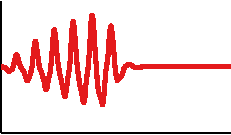
\includegraphics[width=0.2\textwidth]{figures/trans_samples/draw_41} &
      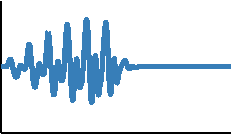
\includegraphics[width=0.2\textwidth]{figures/trans_samples/draw_42} &
      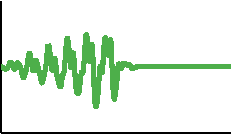
\includegraphics[width=0.2\textwidth]{figures/trans_samples/draw_43} &
      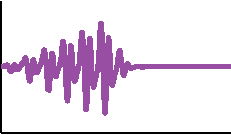
\includegraphics[width=0.2\textwidth]{figures/trans_samples/draw_44}
    \end{tabular}
  \end{block}
\end{frame}

\begin{frame}{Visit our website - try the (simpler) demo}
  \begin{center}
    \Huge www.automaticstatistician.com
  \end{center}
\end{frame}

\end{document}

\begin{frame}{Title}
  \begin{itemize}
    \item Content
    \vspace{\baselineskip}
    \item Content
    \vspace{\baselineskip}
    \item Content
    \begin{itemize}
       \item Content
       \item Content
     \end{itemize}
  \end{itemize}
\end{frame}